\documentclass[10pt]{article}
\usepackage{../../local}


\newcommand{\classcode}{Physics 105}
\newcommand{\classname}{Analytic Mechanics}
\renewcommand{\maketitle}{%
\hrule height4pt
\large{Eric Du \hfill \classcode}
\newline
\large{HW 11} \Large{\hfill \classname \hfill} \large{\today}
\hrule height4pt \vskip .7em
\normalsize
}
\linespread{1.1}
\begin{document}
	\maketitle
	\section*{Collaborators}
	I worked with \textbf{Andrew Binder} and \textbf{Adarsh Iyer} to complete this assignment. 
	\section*{Problem 1}
	Determine the Hamiltonian and Hamilton's equations for the double Atwood machine given in Homework 2 
	Problem 4.

	\begin{solution}
		For this problem, let the height of masses 1 and 2 be $m_1$ and $m_2$, and the height of the pulley be
		$X$. From the previous homeworks, we know that: 
		\[
		\mathcal L = T - U = \frac{1}{2}m_1\dot x_1^2 + \frac{1}{2}m_2\dot x_2^2 +
		\frac{1}{2}m\left( \frac{\dot x_1 + \dot x_2}{2} \right)^2 - m_1gx_1 - m_2gx_2 +
		Mg\left( \frac{x_1 + x_2}{2} \right) 
		\] 
		Then, since we're in a natural coordinate system, we know that $\mathcal H = T + U$, therefore: 
		\[
		\mathcal H = T + U = \frac{1}{2}m_1\dot x_1^2 + \frac{1}{2}m_2\dot x_2^2 +
		\frac{1}{2}m\left( \frac{\dot x_1 + \dot x_2}{2} \right)^2 + m_1gx_1 + m_2gx_2 -
		Mg\left( \frac{x_1 + x_2}{2} \right) 
		\] 
		Then, using $p_i = \pdv{\mathcal L}{\dot q_i}$, we get the system of equations:
		\begin{align*}
			p_1 &= m_1\dot x_1 + \frac{M}{4}(\dot x_1 + \dot x_2) \\
			p_2 &= m_2\dot x_2 + \frac{M}{4}(\dot x_1 + \dot x_2)
		\end{align*}
		Multiplying these equations by 4 so we don't have to deal with fractions, we get: 
		\begin{align*}
			4p_1 &=  \dot x_1 (4m_1 + M) + M\dot x_2 \\
			4p_2 &= \dot x_2(4m_2 + M) + M \dot x_1
		\end{align*}
		Solving this system of equations, we get: 
		\begin{align*}
			\dot x_1 = \frac{p_1(4m_2 + M) - Mp_2}{4m_2m_1 + M(m_2 + m_1)}\\
			\dot x_2 = \frac{p_2(4m_1 + M) - Mp_1}{4m_1m_2 + M(m_1 + m_2)}
		\end{align*}
		Therefore, the Hamiltonian becomes:
		\begin{multline*}
			H = \frac{1}{2}m_1\left[\frac{p_1(4m_2 + M) - Mp_2}{4m_2m_1 + M(m_2 + m_1)}\right]^2 + \frac{1}{2}m_2\left[\frac{p_2(4m_1 + M) - Mp_1}{4m_1m_2 + M(m_1 + m_2)}\right]^2 +\\ \frac{1}{2}M\left[ \frac{4(p_1m_2 + p_2m_1) - M(p_2 + p_1)}{2(4m_2m_1 + M(m_1 + m_2))}\right]^2 +m_1gx_1 + m_2gx_2 - Mg\left( \frac{x_1 + x_2}{2} \right) 
		\end{multline*}
		Now, Hamilton's equations means that we have to find $\pdv{\mathcal H}{p_i}$. Therefore:
		\begin{multline*}
			\dot x_1 = \pdv{\mathcal H}{p_1} = m_1\left[\frac{p_1(4m_2 + M) - Mp_2}{4m_2m_1 + M(m_2 + m_1)}\right] \cdot \frac{4m_2 + M}{4m_2m_1 + M(m_1 + m_2)} -\\ m_2\left[\frac{p_2(4m_1 + M) - Mp_1}{4m_1m_2 + M(m_1 + m_2)}\right] \cdot \frac{M}{4m_2m_1 + M(m_1 + m_2)} +\\ M \left[ \frac{4(p_1m_2 + p_2m_1 - M(p_2 + p_1)}{2(4m_2m_1 + M(m_1 + m_2))}\right] \cdot \frac{4m_2 - M}{2(4m_2m_1 + M(m_1 + m_2))}
		\end{multline*}
		With the power of Mathematica, this simplifies to: 
		\[
			\dot x_1 = \frac{4m_2p_1 + M(p_1 - p_2)}{4m_1m_2 + M(m_1 + m_2)} 
		\] 
		also, the equations here are symmetric in the sense that for $\dot x_2$, it's going to be the expression
		for $x_1$ except we change every $1 \to 2$ and $2 \to 1$, so therefore:
		\[
			\dot x_2 = \frac{4m_1p_2 + M(p_2 - p_1)}{4m_1m_2 + M(m_1 + m_2)}
		\] 
		To get the other two equations we can use the relation $\dot p_i = \pdv{\mathcal H}{q}$:
		\begin{align*}
			\dot p_1 &= \left( \frac{M}{2} - m_1 \right) gx_1\\
			\dot p_2 &= \left( \frac{M}{2} - m_2 \right) gx_2
		\end{align*}
	\end{solution}

	\pagebreak

	\section*{Problem 2}
	Consider a simple plane pendulum of mass $m$ and length $\ell$. After the pendulum is set into motion, the 
	length of the string is shortened at a constant rate. 
	\[
		\dv{\ell}{t} = -\alpha
	\] 
	The suspension point remains fixed. Determine the both Lagrangian and Hamiltonian functions. Compare the 
	Hamiltonian with $E = T + U$, and discuss conservation of energy for this system.

	\begin{solution}
		We write the kinetic energy as $T = \frac{1}{2}m \ell^2 \dot \phi^2 + \frac{1}{2} m \alpha^2$, and the 
		potential energy is $U = -mg\ell\cos\phi$, so therefore the Lagrangian becomes: 
		\[
		\mathcal L = \frac{1}{2}m\ell^2 \dot \phi^2 + \frac{1}{2}m \alpha^2 + mg \ell \cos \alpha
		\] 
		From here, we can get the generalized momenta using $p_i = \pdv{\mathcal L}{\dot q_i}$:
		\begin{align*}
			p_l &= \pdv{\mathcal L}{\dot \ell} = 0 \\
			p_\phi &= \pdv{\mathcal L}{\dot \phi} = m\ell^2 \dot \phi
		\end{align*}
		So now, we can use $\mathcal H = \sum_i p_i q_i - \mathcal L$ to get: 
		\[
		\mathcal H = p_\phi \dot \phi - \left( \frac{1}{2} m\ell^2 \dot \phi^2 + \frac{1}{2}m \alpha^2 + 
		mgl \cos \alpha\right) = \frac{1}{2}m\ell^2 \dot \phi^2 - \frac{1}{2}m \alpha^2 - mgl \cos \phi
		\] 
		Here, we can see that the Hamiltonian isn't the total energy, which is given by $T + U = \frac{1}{2}m
		\alpha^2 + \frac{1}{2}m \ell^2 \dot \phi^2 - mgl \cos \phi$. This is because the Hamiltonian $\mathcal H$ has explicit time dependence, namely in the parameter $l$
		and the fact that $l$ changes in time as $\ell(t) = \ell_0 - \alpha t$, so thus $\pdv{\mathcal H}{t} \neq
		0$.  
	\end{solution}


	\pagebreak

	\section*{Problem 3}
	Consider a particle of mass $m$ constrained to move on a frictionless cylinder of radius $R$, described in 
	cylindrical coordinates by the surface $\rho = R$. The mass is attached to a spring (spring constant $k$
	and equilibrium length zero) whose other end is fastened at the origin. Using cylindrical coordinates, 
	$(\rho, \phi, z)$, find the Hamiltonian $H$. Then write down and solve Hamilton's equations and describe
	the motion.

	\begin{solution}
		Since cylindrical coordinates are natural, we know that the Hamiltonian is just going to be the kinetic
		plus potential energy. Setting the axis to be the origin, we can now write down the kinetic and potential
		energies in cylindrical coordinates:
		\begin{align*}
			T &=  \frac{m}{2}(\dot \rho^2 +\rho^2 \dot \phi^2 + \dot z^2) + \frac{1}{2}(R^2 \dot \phi^2 + z^2)\\
			V &= \frac{1}{2}kr^2 = \frac{1}{2}k(R^2 + z^2)
		\end{align*}
		We can cancel the $\dot \rho$ terms since the mas sis constrained to move on the cylinder. Therefore, 
		we have: 
		\[
		\mathcal H = T + V = \frac{m}{2}(R^2 \dot \phi^2 + \dot z^2) + \frac{k}{2}(R^2 + z^2)
		\] 
		Computing the generalized momenta using $p_i = \dv{T}{q_i}$, since we're working in natural 
		coordinates :
		\begin{align*}
			p_z &=  \dv{T}{\dot z} = m\dot z \\
			p_\phi &= \dv{T}{\dot \phi} = mR^2 \dot \phi
		\end{align*}
		So Hamilton's equation then becomes:
		\[
			\mathcal H = \frac{m}{2}\left(R^2 \frac{p_{\phi}^2}{(mR^2)^2} + \frac{p_z^2}{m^2}\right) + 
			\frac{k}{2}(R^2 + z^2) = \frac{p_\phi^2}{2mR^2} + \frac{p_z^2}{2m} + \frac{k}{2}(R^2 + z^2)
		\] 	

		Finally, we can write Hamilton's equations:
		\begin{align*}
			\dot \phi &= \pdv{\mathcal H}{p_\phi} = \frac{p_\phi}{2mR^2}\\
			\dot z &= \pdv{\mathcal H}{p_z} = \frac{p_z}{m}\\
			\dot p_\phi &= -\pdv{\mathcal H}{\phi} = 0\\
			\dot p_z &= -\pdv{\mathcal H}{z} = -kz
		\end{align*}
		These then give us our equations of motion. Since $\dot p_\phi = 0$, this implies that $p_\phi$ is a
		constant, and thus $\dot \phi$, which is defined in terms of $p_\phi$, is also a constant. In the $z$
		direction, we have 
		\[
			\dot z = \frac{p_z}{m} \implies \ddot z = -\frac{k}{m} z
		\] 
		And so we get $z(t) = A\cos(\omega t - \delta)$, where $A, \delta$ are some constants  given by initial 
		conditions. 

		In terms of the motion of the particle, we see that it oscillates sinusoidally in the $z$ direction, 
		and moves around in the $\hat{\phi}$ direction with a uniform velocity. This makes intuitive 
		sense as well, since the spring force always acts perpendicular to $\hat{ \phi}$, so we don't expect
		any change in velocity in that direction. The same cannot be said for the $z$ direction, which is why
		we sinusoidal oscillations. 
	\end{solution}


	\pagebreak

	\section*{Problem 4}
	Consider the modified Atwood machine shown in Figure 13.11. The two weights on the left have equal mass $m$
	and are connected by a massless spring of force constant $k$. The weight on the right has mass $M = 2m$,
	and the pulley is massless and frictionless. The coordinate $x$ is the extension of the spring from 
	its equilibrium length; that is, the length of the spring is $l_e + x$, where $l_e$ is the equilibrium
	length (with all the weights in position $M$ held stationary). 

	\begin{enumerate}[label=\alph*)]
		\item Show that the total potential energy (spring plus gravitational) is just $U = \frac{1}{2}kx^2$
			(plus a constant that can be taken to zero). 

			\begin{solution}
				Using the position of the big wheel as zero potential energy, we can write the gravitational potential
				energy in the system as:
				\[
					U_g = -mgy - mg(y + l_e + x) - Mg(L - y) = mg(y + y + l_e + x + 2(L - y) = -mgx + \text{const.}
				\] 
				Then, to express spring potential energy, let $l_0$ denote the natural length of the spring. 
				From balancing of forces, we see that: 
				\[
				k(le - l_0) = mg
				\] 
				Then, we can now calculate the spring potential energy:
				\[
				U_s = \frac{1}{2}k(x + le - l_0)^2 = \frac{1}{2}k\left( x + \frac{mg}{k} \right)^2 = \frac{1}{2}
				kx^2 + mgx + \frac{1}{2}k^3
				\] 
				Combining the two expressions now:
				\[
					U_g + U_s = \frac{1}{2}kx^2 + mgx + \frac{1}{2}k^3 - mgx - \text{const.}
				\] 
				Since $\frac{1}{2}k^3$ is also a constant and the $mgx$ terms cancel, then we see that the total
				energy in the system is indeed equal to $\frac{1}{2}kx^2$ plus a constant. 
			\end{solution}
		\item Find the two momenta conjugate to $x$ and $y$. Solve for $\dot x$ and $\dot y$ and write down 
			the Hamiltonian. Show that the coordinate $y$ is ignorable. 

			\begin{solution}
				Here, since the coordinate system is natural, we can find $p_i$ by taking $\dv{T}{\dot q_i}$. 
				First, calculating $T$:
				\[
				T = \frac{1}{2}M \dot y^2 + \frac{1}{2}my^2 + \frac{1}{2}m(\dot x + \dot y)^2 =
				\frac{3}{2}m\dot y^2 + \frac{1}{2}m(\dot x + \dot y)^2
				\] 
				therefore, we can now get $p_i$: 
				\begin{align*}
					p_x &= \pdv{T}{\dot x} = m(\dot x + \dot y)\\
					p_y &= \pdv{T}{\dot y} = 3m \dot y + m(\dot x + \dot y)
				\end{align*}	
				From these equations, we can then backsolve for $\dot y$ and $\dot x + \dot y$ 
				\begin{align*}
					\dot x + \dot y &= \frac{p_x}{m}\\
					\dot y &= \frac{p_y - p_x}{3m}
				\end{align*} 
				Therefore, the Hamiltonian written in these coordinates is:
				\[
					\mathcal H = T + U = \frac{1}{2}m\left[ \frac{p_x^2}{m^2} + \frac{(p_y - p_x)^2}{m^2}\right] 
					+ \frac{1}{2}kx^2
				\] 
				Since $\pdv{\mathcal H}{y} = 0$, then this means that $y$ is an ignorable coordinate. 
			\end{solution}
		\item Write down the four Hamilton equations and solve them for the following initial conditions: You
			hold the mass $M$ fixed with the whole system in equilibrium and $y = y_0$. Still holding $M$ fixed,
			you pull the lower mass $m$ a distance $x_0$, and at $t = 0$ you let go of both masses. 
			[\textit{Hint:} Write down the initial values $x$, $y$ and their momenta. You can solve the $x$ 
			equations by combining them into a second-order equation for $x$. Once you know $x(t)$, you can 
			quickly write down the other three variables.] Describe the motion. In particular, find the frequency
			with which $x$ oscillates. 


			\begin{solution}
				The four Hamilton equations come from just taking derivatives:
				\begin{align*}
					\dot x &= \pdv{\mathcal H}{p_x} = \frac{1}{3m}(4p_x - p_y)\\
					\dot y &= \pdv{\mathcal H}{p_y} = \frac{p_y - p_x}{3m}\\
					\dot p_x &= -\pdv{\mathcal H}{ x} = -kx\\
					\dot p_y &= -\pdv{\mathcal H}{y} = 0
				\end{align*}

				Since we hold $M$ fixed, then this also means that we're holding the mass on the other side
				to be fixed as well. This gives the initial conditions: $\dot x(0) = 0$ and $\dot y(0) = 0$, 
				implying that $p_x(0) = p_y(0) = 0$. Further, from Hamilton's equations, we can find $\ddot x$
				\[
				\ddot x = \frac{1}{3m}(4 \ddot p_x - \ddot p_y) = \frac{4k}{3m}x
				\] 
				This is the same equation of motion as a harmonic oscillator, so therefore $x$ oscillates with 
				frequency $\omega = \sqrt{\frac{4k}{3m}}$. Therefore: 
				\[
				x(t) = x_0\cos(\omega t)
				\] 
				As for the other coordinates, since we know that $\dot p_x = kx$, then: 
				\[
				p_x(t) = \frac{kx_0}{\omega}\sin(\omega t)
				\] 
				Finally, we can get $y(t)$ using $\dot y = -\frac{p_x}{3m}$:
				\[
				y(t) = \frac{1}{3m}\frac{x_0}{\omega}\cos(\omega t) + y_0
				\] 

			\end{solution}
	\end{enumerate}


	\pagebreak

	\section*{Problem 5}
	A spherical pendulum consists of a mass $m$ attached to a massless, rigid rod of length $\ell$. The end 
	of the rod opposite the mass can pivot freely (hence ``spherical" pendulum) in all directions about
	some fixed point. 

	\begin{enumerate}[label=\alph*)]
		\item Set up the Hamiltonian function (in spherical coordinates!). Check that if $p_\phi = 0$, the
			result is the same as that for a plane pendulum. 

			\begin{solution}
				To set up the Hamiltonian, we again use the fact that our coordinate system is natural, so the 
				Hamiltonian in this case will just be the sum of our potential and kinetic energies. Writing
				this out in spherical coordinates, we get: 
				\begin{align*}
					T = \frac{1}{2}m(\dot r^2 + \ell^2 \dot \theta^2 + \ell^2 \sin^2 \theta \dot \phi^2) = \frac{m}{2}\left( \ell^2 \dot \theta^2 + \ell^2 \sin^2 \theta \dot \phi^2 \right) 
					V = mg \cos \theta
				\end{align*}
				We drop the $\dot \ell$ term because the rod is rigid, so there is no change radially. Now
				writing out the generalized momentum using $p_i = \dv{T}{\dot q_i}$ (again, we can do this
				because our coordinate system is natural):
				\begin{align*}
					p_{\theta} &= \pdv{T}{\dot \theta} = m \ell^2 \dot \theta  \implies \dot \theta 
					= \frac{p_\theta}{m\ell^2}\\
					p_{\phi} &= \pdv{T}{\dot \phi} = m\ell^2 \sin^2 \theta \dot \phi \implies \dot \phi = \frac{p_\phi}{m\ell^2 \sin^2 \theta} 
				\end{align*}
				So therefore, we can rewrite $T$:
				\[
					T = \frac{1}{2m\ell^2}\left( p_\theta^2 + \frac{p_\phi^2}{\sin^2 \theta} \right) 
				\] 
				In the case where $p_\phi = 0$, then the second term in the parentheses goes to zero, so 
				therefore we're left with: 
				\[
					\mathcal H = \frac{p_\theta^2}{2m\ell^2} + mg \cos \theta
				\] 
				Which is the exact equation for a plane pendulum. 
			\end{solution}
		\item Combine the term that depends on $p_\phi$ with the ordinary potential energy term to define an 
			effective potential $V(\theta, p_\phi)$. Sketch $V$ as a function of $\theta$ for several values of 
			$p_\phi$, making sure to include $p_\phi = 0$.


			\begin{solution}
				Rewirting the Hamiltonian a bit: 
				\[
					\mathcal H = \frac{p_\theta^2}{2m\ell^2} + \frac{p_\phi^2}{2m\ell^2 \sin^2 \theta} + 
					mg \cos \theta 
				\] 
				Then it's clear that if we want only the $p_\theta$ term to remain, then we would want the 
				effective potential to be 
				\[
					V(\theta, p_\phi) = \frac{p_\phi^2}{2m\ell^2 \sin^2 \theta} + mg \cos \theta
				\] 
				The sketches for $V(\theta, p_\phi)$ for $\theta \in [0, \pi]$ are shown below, first for
				$p_\phi = 1, 3, 6, 10$ in that
				order, from left to right:
				\begin{center}
					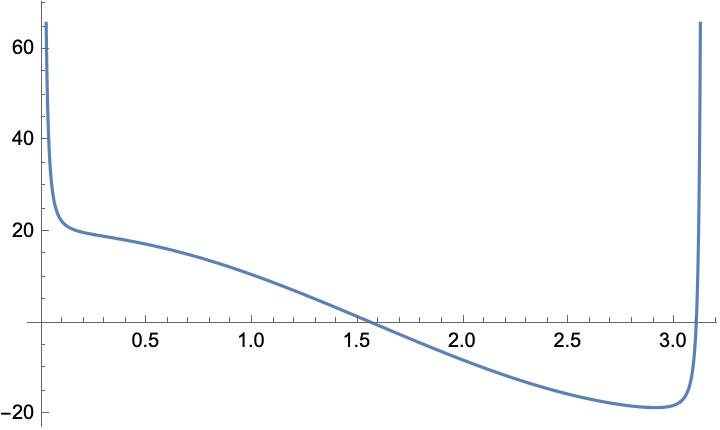
\includegraphics[width = 0.23\textwidth]{q5plot1.jpeg}
					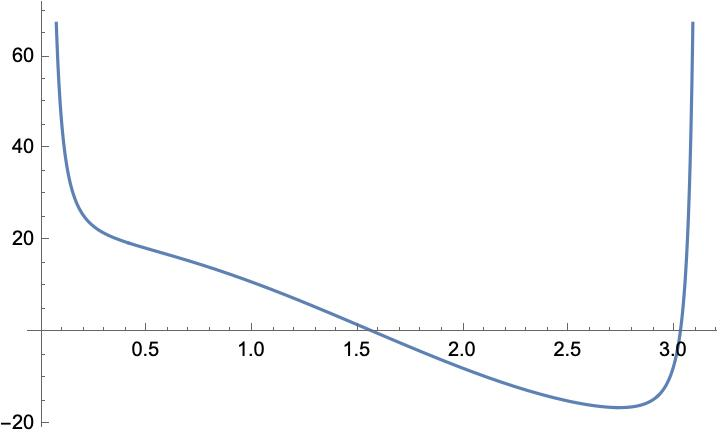
\includegraphics[width = 0.23\textwidth]{q5plot2.jpeg}
					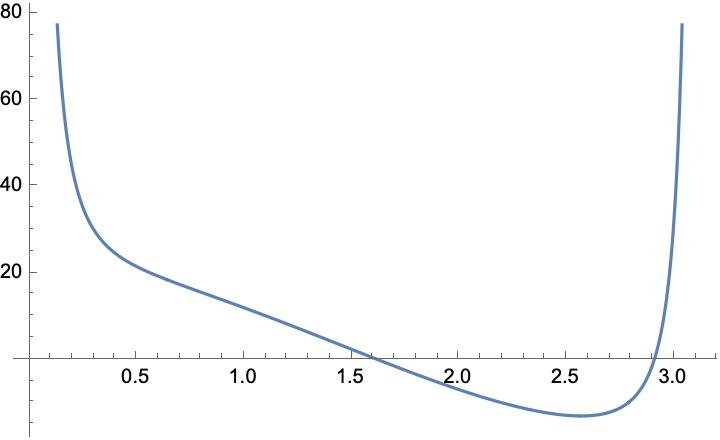
\includegraphics[width = 0.23\textwidth]{q5plot3.jpeg}
					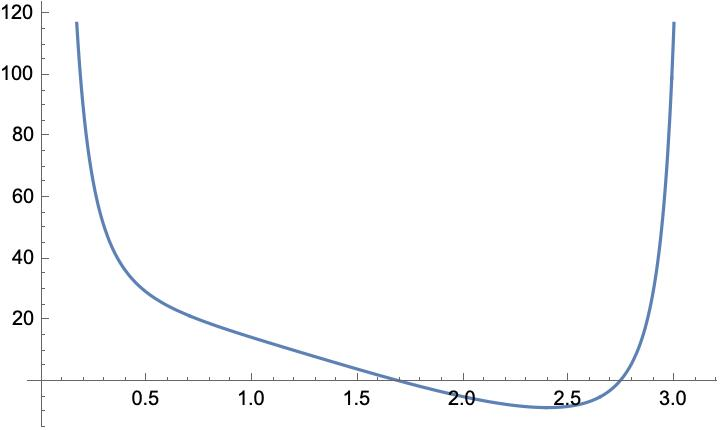
\includegraphics[width = 0.23\textwidth]{q5plot4.jpeg}
				\end{center}
				For $p_\phi = 0$, this is what we get over the same interval $\theta \in [0, \pi]$:
				\begin{center}
					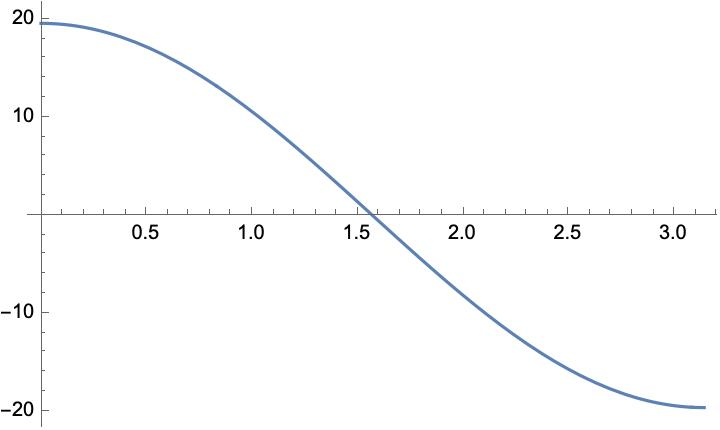
\includegraphics[scale=0.8]{q5plot5.jpeg}
				\end{center}
			\end{solution}
		\item Discuss the features of the motion, pointing out the differences between $p_\phi = 0$ and 
			$p_\phi \neq 0$. Discuss the limiting case of the conical pendulum, $\theta = C$, a constant, with
			reference to the $V-\theta$ diagram. 


			\begin{solution}
				Firstly, the motion looks very different for $p_\phi = 0$ as opposed to $p_\phi \neq 0$. 
				Perhaps the most noticeable difference is the fact that with the case where $p_\phi \neq 0$, 
				we get a global minimum at a $\theta \in (0, \pi)$, whose specific value is determined by 
				$p_\phi$ itself. In the case where $p_\phi = 0$, we get a global minimum at $\theta = \pi$ --
				this makes sense, since there is no angular component to ``carry'' the mass around the 
				sphere.
				
				In terms of the motion itself: when $p_\phi \neq 0$, then we see that this leads to $\theta 
				\neq 0$, implying that the mass travels around the sphere. For larger values of $p_\phi$, 
				we can see that the local minimum of the curve approaches $\frac{\pi}{2}$, this corresponds to 
				the point when the mass rotates around the axis horizontally.
				
				To analyze the conical pendulum, it's useful to first notice that $\pdv{\mathcal H}{\phi} = 0$,
				so therefore $p_\phi$ is a constant. 
				Because of this, it means that the pendulum will circulate the vertical axis about which
				the pendulum is rotating with both a constant polar angle and constant azimuthal angular velocity
				In other words, $\dot \phi$ is a constant throughout the motion.
			\end{solution}
	\end{enumerate}
\end{document}


